\documentclass[showpacs, oneside, onecolumn, prl, amsmath, amssymb, nofootinbib, superscriptaddress, notitlepage]{revtex4-1}


\usepackage{cases}
\usepackage{amsmath}
\usepackage{amssymb}
\usepackage{amsfonts}
\usepackage{amssymb}
\usepackage{dcolumn}
\usepackage{bm}
\usepackage{bbm}
\usepackage{graphicx}
\usepackage{xcolor}
\usepackage{array}
\usepackage{subfigure}
\usepackage{hyperref}
\usepackage{multirow}
\usepackage{ulem}

%%%%%%%%%%%%%%%%%%%%%%%%%%%%%%%%%%%%%%%%%%%%%%%%%%%%%%%%%%%%%%%%%%%%%%%%%%%%%%%%%%%
\newcommand{\bra}[1]{\langle #1\vert}
\newcommand{\ket}[1]{\vert #1\rangle}
\newcommand{\nn}{\nonumber \\}
\newcommand{\lag}{\langle}
\newcommand{\rag}{\rangle}
\newcommand{\cN}{{\cal N}}
\newcommand{\cA}{{\cal A}}
\newcommand{\gsim}{\mathrel{\hbox{\rlap{\lower.55ex \hbox {$\sim$}}
                   \kern-.3em \raise.4ex \hbox{$>$}}}}
\newcommand{\lsim}{\mathrel{\hbox{\rlap{\lower.55ex \hbox {$\sim$}}
                   \kern-.3em \raise.4ex \hbox{$<$}}}}

\newcommand\be{\begin{equation}}
\newcommand\ba{\begin{align}}
\newcommand\bas{\begin{align*}}
\newcommand\bt{\begin{table}}
\newcommand\bts{\begin{table*}}
\newcommand\bfig{\begin{figure}}
\newcommand\bfs{\begin{figure*}}
\newcommand\ee{\end{equation}}
\newcommand\ea{\end{align}}
\newcommand\et{\end{table}}
\newcommand\ets{\end{table*}}
\newcommand\efig{\end{figure}}
\newcommand\efs{\end{figure*}}
\newcommand\RA{$\ \ \Rightarrow\ \ $}


\newcommand\blue{\textcolor{blue}}
\newcommand\gray{\textcolor{gray}}
\newcommand\green{\textcolor{teal}}
\newcommand\red{\textcolor{red}}




\hypersetup{colorlinks=true,
            breaklinks=true,
            pdfstartview=Fit,
            linkcolor=blue,
            citecolor=green,
            urlcolor=blue}

\bibliographystyle{apsrev4-1}




%%%%%%%%%%%%%%%%%%%%%%%%%%%%%%%%%%%%%%%%%%%%%%%%%%%%%%%%%%%%%%%%%%%%%%%%%%%%%%%%%%%
\begin{document}
	
\title{Problem Set 6}

\author{JIAO Hao}

\maketitle

~~~~

%%%%%%%%%%%%%%%%%%%%%%%%%%%%%%%%%%%%%%%%%%%%%%%%%%%%%%%%%%%%%%%%%%%%%%%%%%%%%%%%%%%
\section{Problem 1}

%------
\bfig
	\centering
	\subfigure
	{\begin{minipage}[b]{0.39\textwidth}
	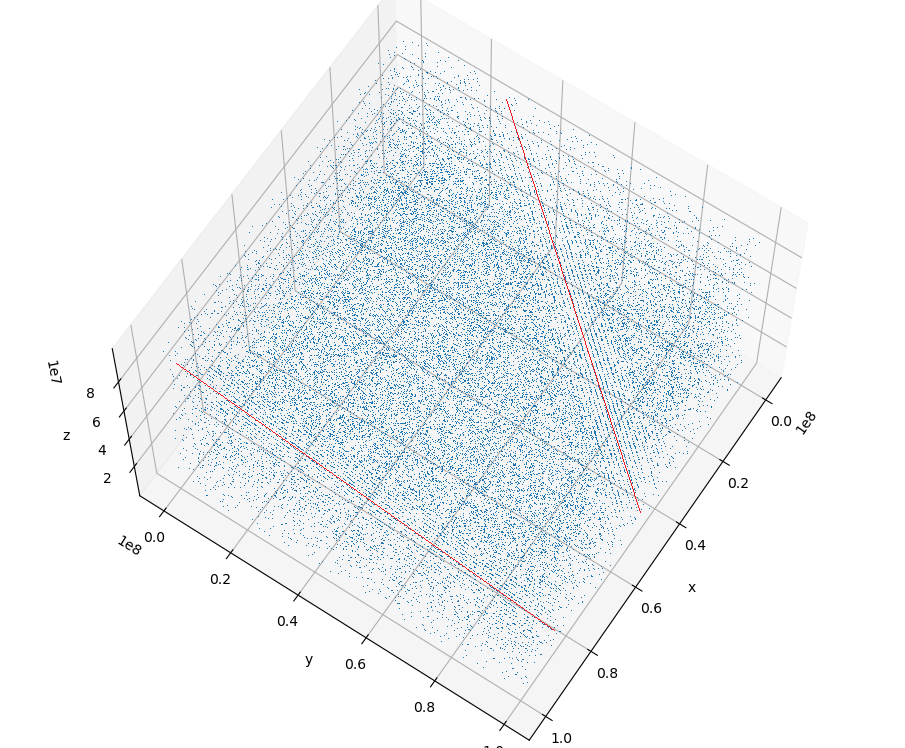
\includegraphics[scale=0.4]{6-1-1.png}
	\end{minipage}}
	\subfigure
	{\begin{minipage}[b]{0.39\textwidth}
	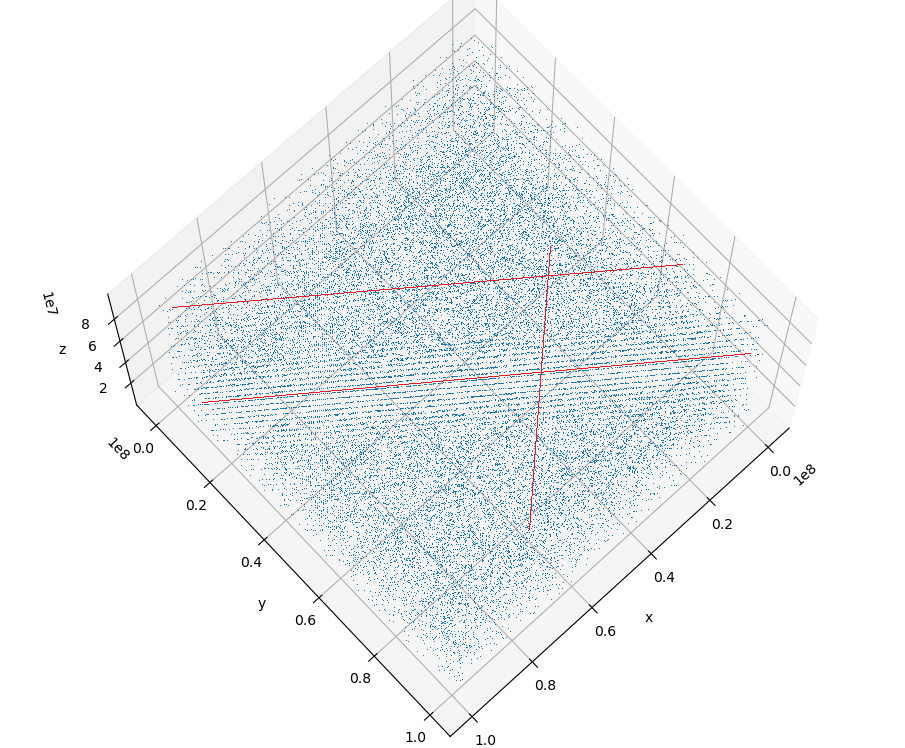
\includegraphics[scale=0.4]{6-1-2.png}
	\end{minipage}}
	\subfigure
	{\begin{minipage}[b]{0.39\textwidth}
	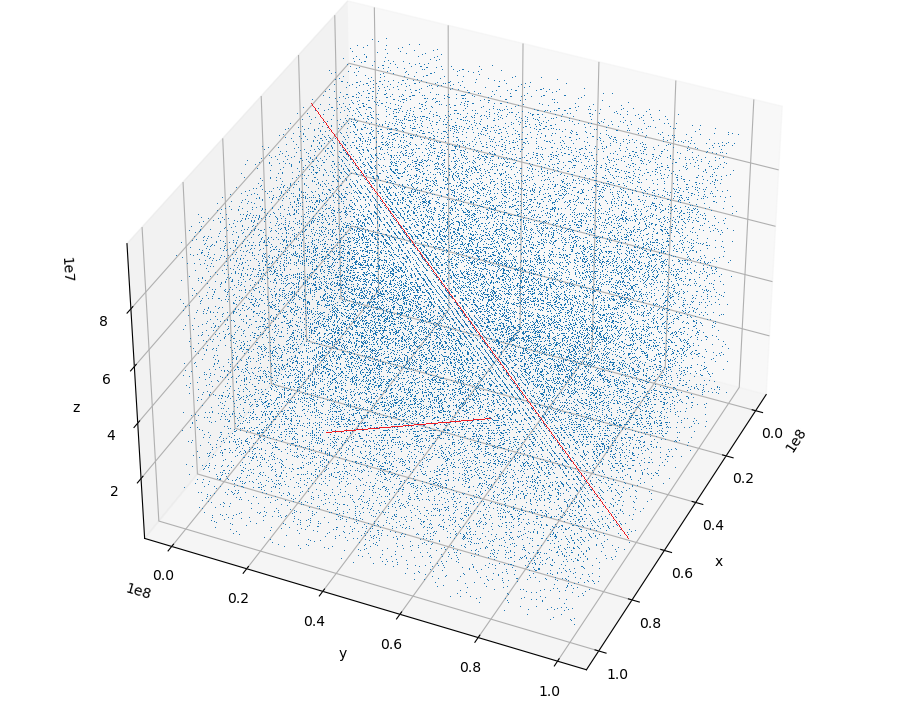
\includegraphics[scale=0.4]{6-1-3.png}
	\end{minipage}}
	\subfigure
	{\begin{minipage}[b]{0.39\textwidth}
	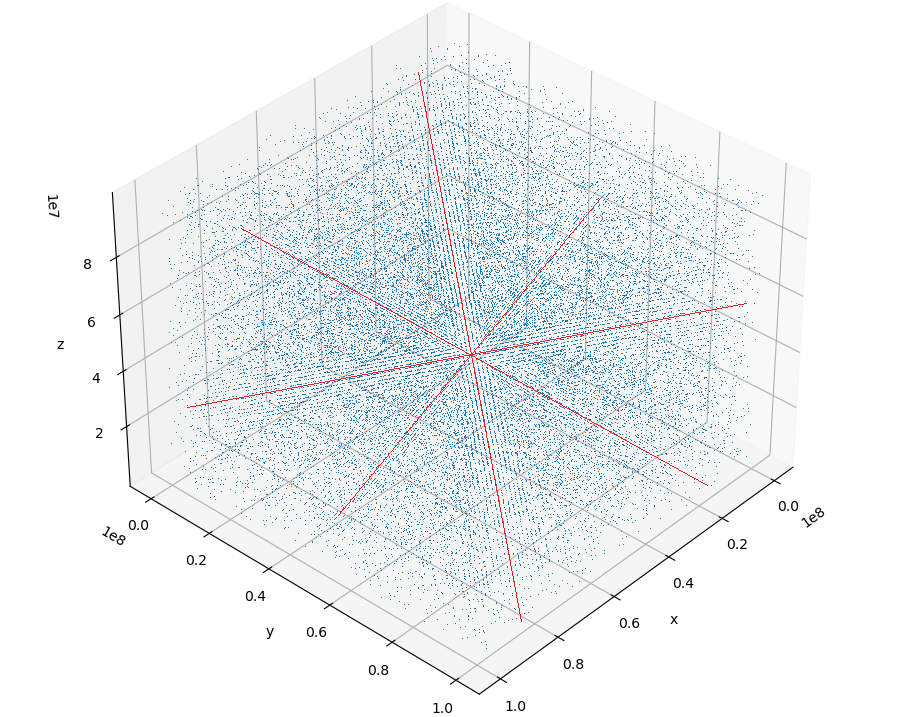
\includegraphics[scale=0.4]{6-1-4.png}
	\end{minipage}}
	\subfigure
	{\begin{minipage}[b]{0.39\textwidth}
	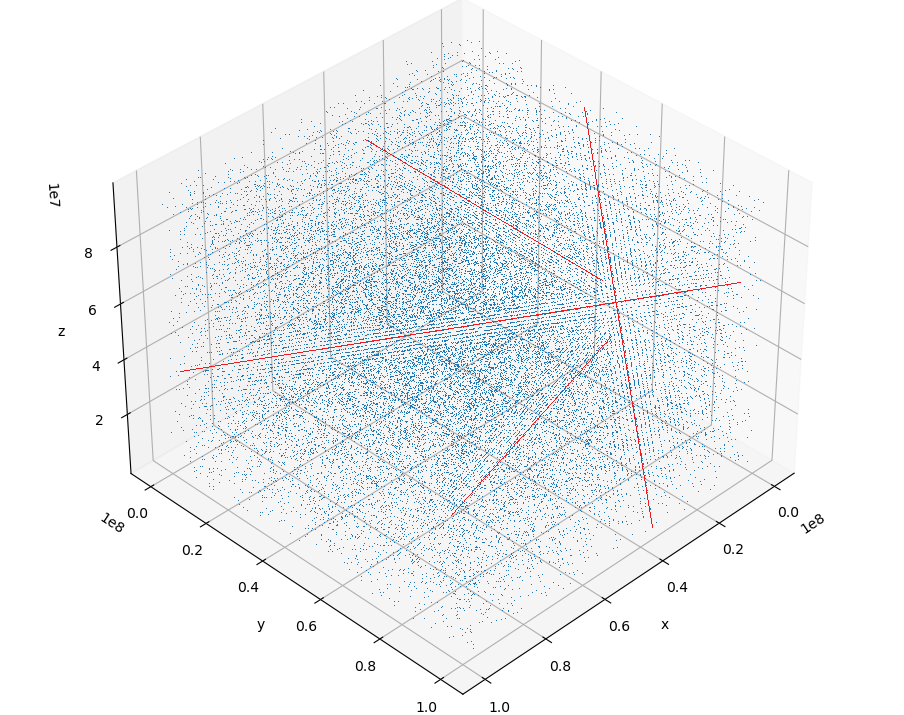
\includegraphics[scale=0.4]{6-1-5.png}
	\end{minipage}}
	\subfigure
	{\begin{minipage}[b]{0.39\textwidth}
	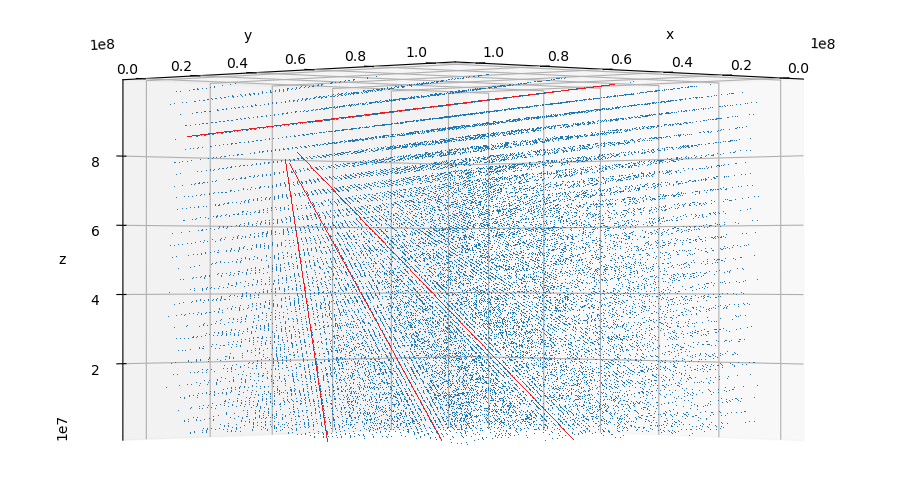
\includegraphics[scale=0.4]{6-1-6.png}
	\end{minipage}}
	\subfigure
	{\begin{minipage}[b]{0.39\textwidth}
	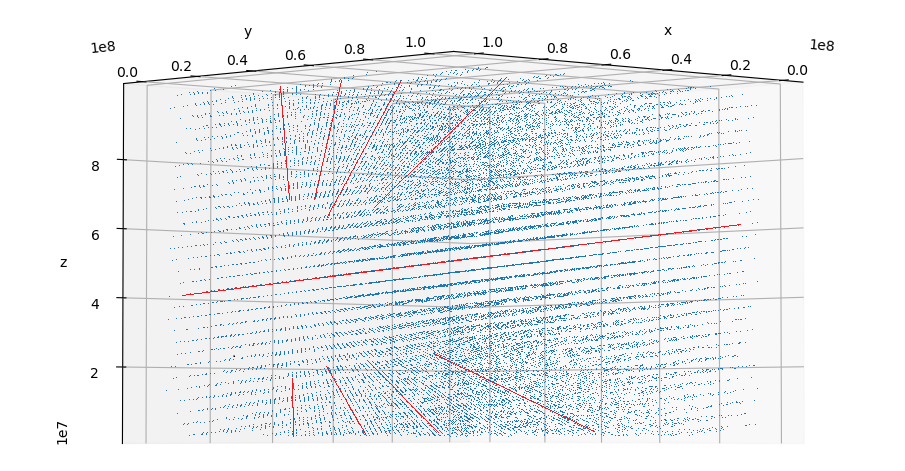
\includegraphics[scale=0.4]{6-1-7.png}
	\end{minipage}}
	\subfigure
	{\begin{minipage}[b]{0.39\textwidth}
	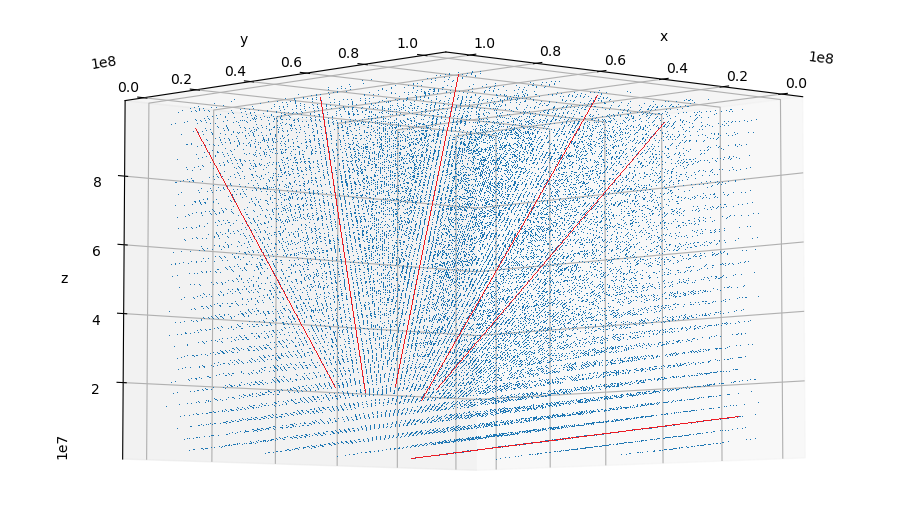
\includegraphics[scale=0.4]{6-1-8.png}
	\end{minipage}}
	\caption{Show that these `random points' by the random number generator in the C standard library are in some planes. I denotes these planes by red lines. If these figures are not clear enough, you can see them in the files named `6-1-1.png' to `6-1-8.png'.}
	\label{6-1}
\efig

%------
\bfig
	\centering
	\subfigure
	{\begin{minipage}[b]{1\textwidth}
	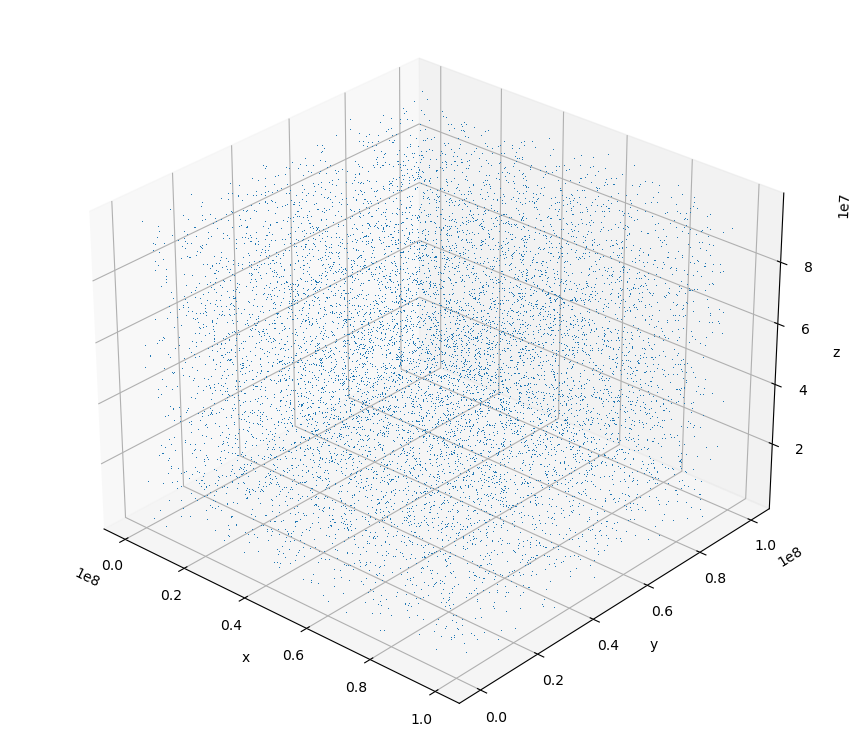
\includegraphics[scale=0.6]{6-1-python.png}
	\end{minipage}}
	\subfigure
	{\begin{minipage}[b]{1\textwidth}
	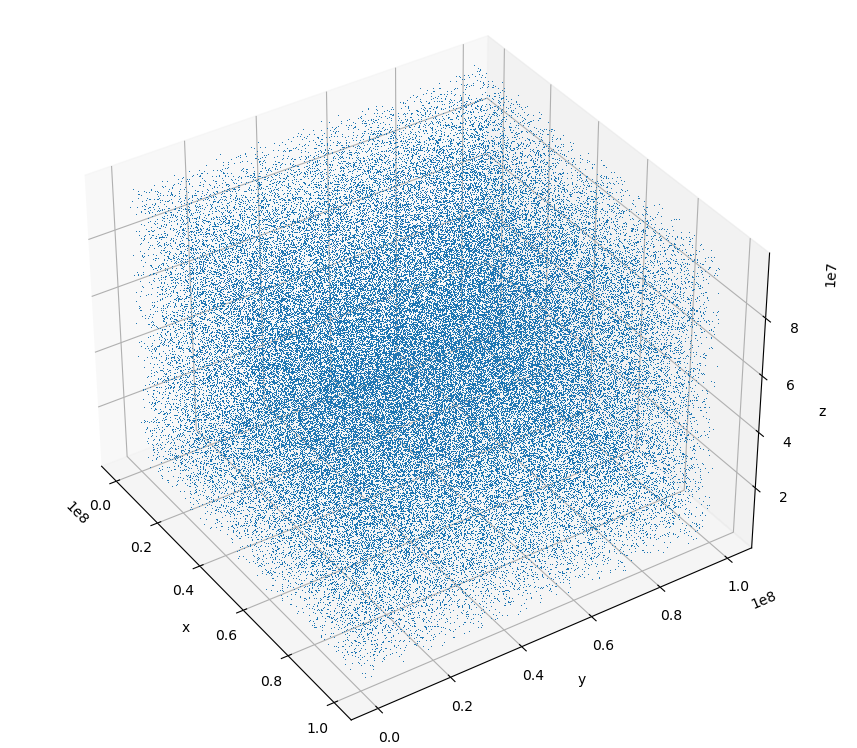
\includegraphics[scale=0.6]{6-1-python1.png}
	\end{minipage}}
	\caption{Random points generated by python random number generator.}
	\label{6-1-2}
\efig


We can find from fig.\ref{6-1} that the `random numbers (vectors)' producted by C standard library are lying on some planes and they are very much not randomly distributed in 3D space. 

But I got more planes than professor: at least 35 horizontal plane (shown in ``6-1-7.png''), and there also are planes with other derection (three direction should be the same).

~~~~

I didn't successfully run the library of python (``JIAO Hao-6-1-1''). But I think the ramdom number generated by python is good. I show 10000 and 100000 ramdom points generated by ``1e8*np.random.rand(n)'' in the same volume as above, and we can see that they are really random (``JIAO Hao-6-1-1'', and fig.\ref{6-1-2}).


~~~~

~~~~

%%%%%%%%%%%%%%%%%%%%%%%%%%%%%%%%%%%%%%%%%%%%%%%%%%%%%%%%%%%%%%%%%%%%%%%%%%%%%%%%%%%
\section{Problem 2}

%%%%%%%%%%%%%%%%%%%%%%%%%%%%%%%%%%%%%%%%
\textbf{Which of Lorentzians, Gaussians, and power laws could you use for the bounding distribution?}

If the distribution is bounded in $[0,a]$, we can use all three distribution to get the exponential deviates. But if we consider the distribution at $[0,\infty]$, we can only use Lorentzians and power laws:
\bas
&\lim_{x\rightarrow\infty}\frac{\exp[x/\tau]}{\tau}/\frac{1}{\pi(1+x^2)}=0\\
&\lim_{x\rightarrow\infty}\frac{\exp[x/\tau]}{\tau}/\frac{\exp[-x^2/2\sigma^2]}{\sqrt{2\pi\sigma}}=\infty\\
&\lim_{x\rightarrow\infty}\frac{\exp[x/\tau]}{\tau}/(\alpha+1)x^\alpha=0
\end{align*}

I use both Lorentzians and power laws:

Form Lorentzian:

\gray{The accept rate from Lorentz to Exponential deviates is 6365045 / 9366561 = 0.6795498369145303}

\gray{Transformation method use 0.22466683387756348 s.}

\gray{The rejection method use 1.4030277729034424 s.}~~~~

Form power laws:

\gray{The accept rate from PowerLaw to Exponential deviates is 7034369 / 9500645 = 0.7404096248202096}

\gray{Transformation method use 0.25522756576538086 s.}

\gray{The rejection method use 1.9982857704162598 s.}

~~~~

\textbf{The histogram of my deviates matches up with the expected exponential curve}

%------
\bfig
	\centering
	\subfigure
	{\begin{minipage}[b]{1\textwidth}
	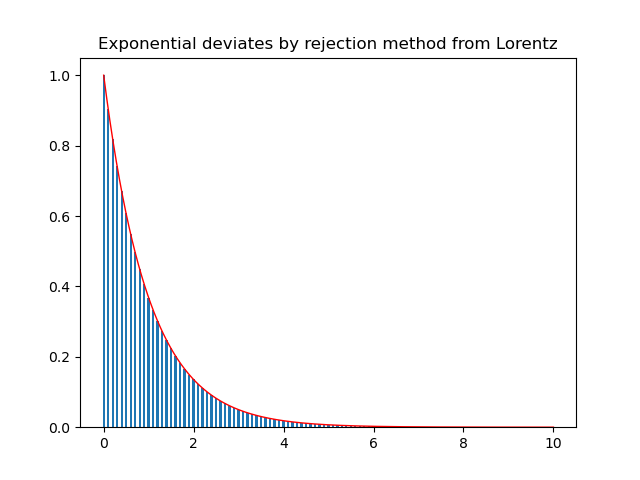
\includegraphics[scale=0.8]{6-2-1.png}
	\end{minipage}}
	\subfigure
	{\begin{minipage}[b]{1\textwidth}
	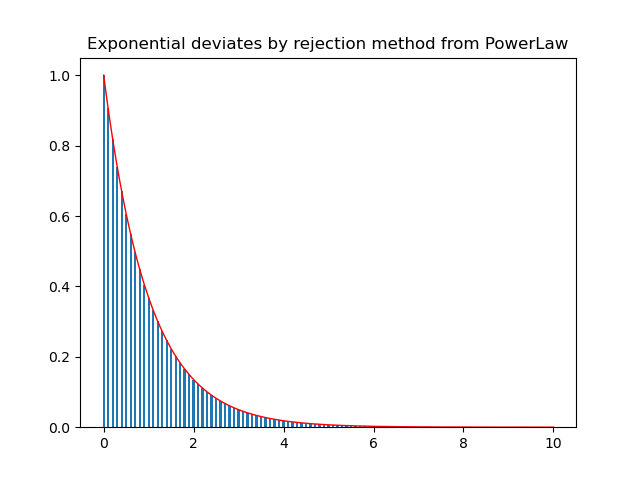
\includegraphics[scale=0.8]{6-2-2.png}
	\end{minipage}}
	\caption{Generate exponential deviates from another distribution by rejection method}
	\label{6-2}
\efig

Shown in fig.\ref{6-2}. We can see that both the two distribution matched the expected exponential curve very well.

~~~~

\textbf{How efficient can you make this generator, in terms of the fraction of uniform deviates that give rise to an exponential deviate?}

\gray{The accept rate from Lorentz to Exponential deviates is 6365045 / 9366561 = 0.6795498369145303}

\gray{The accept rate from PowerLaw to Exponential deviates is 7034369 / 9500645 = 0.7404096248202096}

\gray{The accept rate from Uniform to Exponential deviates is 1001223 / 10000000 = 0.1001223}


~~~~

~~~~

%%%%%%%%%%%%%%%%%%%%%%%%%%%%%%%%%%%%%%%%%%%%%%%%%%%%%%%%%%%%%%%%%%%%%%%%%%%%%%%%%%%
\section{Problem 3}

Since the random number with exponential distribution is alway positive, we shuold keep $v/u>0$ \RA $v\in [0,1]$ rather than $v\in[-1,1]$.

%------
\bfig
	\centering
	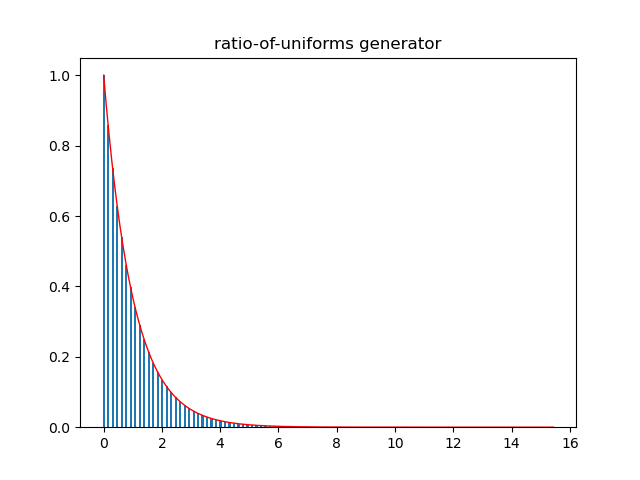
\includegraphics[scale=0.8]{6-3.png}
	\caption{Generate exponential deviates by ratio-of-uniforms generator.}
	\label{6-3}
\efig

The result is shown in fig.\ref{6-3}. From this, we can see that this generator also produces the correct answer.

~~~~

And we can get that the efficiency of this genertor is acceptable:

\gray{The accept rate of ratio-of-uniforms generator is 0.5002858}















\end{document}